% !Rnw root = learnR.Rnw

%% ---preamble.tex----%% 
%% maxwidth is the original width if it is less than linewidth
%% otherwise use linewidth (to make sure the graphics do not exceed the margin)
\makeatletter
\def\maxwidth{ %
  \ifdim\Gin@nat@width>\linewidth
    \linewidth
  \else
    \Gin@nat@width
  \fi
}
\makeatother

\definecolor{fgcolor}{rgb}{0.345, 0.345, 0.345}

\definecolor{shadecolor}{rgb}{.97, .97, .97}
\definecolor{messagecolor}{rgb}{0, 0, 0}
\definecolor{warningcolor}{rgb}{1, 0, 1}
\definecolor{errorcolor}{rgb}{1, 0, 0}






% \subsection*{Australian and New Zealand alcohol consumption}
% 
% \begin{SaveVerbatim}{grogcode}
% ## Simplified version of plot
% form <-
%   Beer+Spirit+Wine ~ Year|Country
% grogplot <- xyplot(form, data=grog,
%                    outer=FALSE)
% ## Enhance, and print enhanced code
% parset <- simpleTheme(pch=c(1,3,4))
% update(grogplot, ylim=c(0,5.5),
%        xlab="",
%        ylab="Amount (per person)",
%        auto.key=list(columns=3)
%        par.settings=parset)
% \end{SaveVerbatim}
% 
% \setkeys{Gin}{width=0.98\textwidth}
% \begin{figure}
% 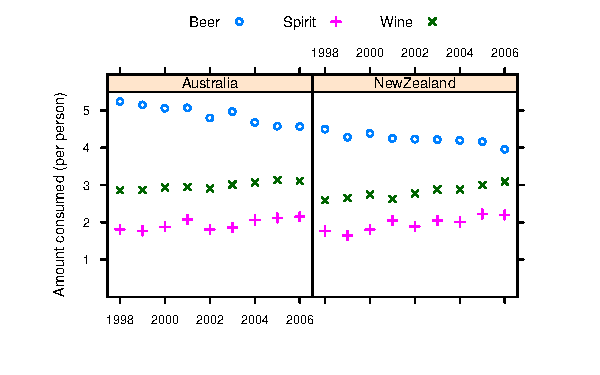
\includegraphics[trim=9 18 0 15]{colorArt/allgrog}%
%   \caption{Australian and New Zealand apparent per person annual
%   consumption (in liters) of the pure alcohol content of liquor products, for
%   1998 to 2006.  This is a color version of Figure \ref{fig:allgrog}.
% version of this graph.
% \protect\UseVerbatim[fontsize=\relsize{-1}]{grogcode}
% \label{col:fig31}}
% \vspace*{18pt}
% \end{figure}
% 
% \subsection*{Height versus weight of Australian athletes}
% \begin{SaveVerbatim}{qplot}
% quickplot(wt, ht, data=aisRS,
%      geom="point", size=I(2),
%      color=sex, shape=sport)
% \end{SaveVerbatim}
% 
% \begin{figure}
% \begin{center}
% \begin{minipage}[c]{0.85\textwidth}
% 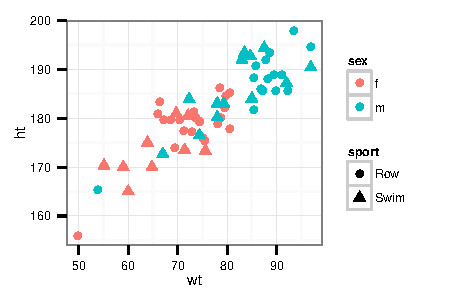
\includegraphics[trim=0 18 0 12]{colorArt/colshape.pdf}
% \end{minipage}
% \end{center}
%   \caption{Here, \texttt{color}s distinguish \texttt{sex}es,
% while \texttt{shape}s distinguish \texttt{sport}s.}\label{col:colshape}
% \setfloatalignment{b}
% \end{figure}
% \marginnote{Code that uses \txtt{quickplot()} is:
% \vspace*{-7pt}
% 
% \UseVerbatim[fontsize=\relsize{-1}]{qplot}
% }
% 
% \newpage
% 
% \subsection*{A color density plot}
% 
% \begin{figure}[h]
% \vspace*{-30pt}
% <<smoothScatter, w=2.75, h=2.85, top=2, echo=FALSE, out.width="0.44\\textwidth">>=
% library(DAAG)
% dfsamp <- cps1[sample(nrow(cps1), 3000), ]
% blueRamp <- colorRampPalette(c("white", blues9))
% with(dfsamp, smoothScatter(re75~re74,
%                            colramp=blueRamp))
% mtext(side=3, line=0.5, "Color density plot", adj=0)
% @ %
% \caption{The function \txtt{smoothScatter()} has been used to give
%   a color density representation of the plot of \txtt{re75} versus
%   \txtt{re74}, for a sample of 3000 rows from the dataset \txtt{cps1}
% ({\em DAAG}).  (Color version of Figure
% \ref{fig:alpha}C).\label{col:alphaC}}
% \vspace*{-12pt}
% \end{figure}
% 
% \enlargethispage{60pt}

\subsection*{Annotated Motion Chart}

\begin{figure*}[h]
\vspace*{-6pt}
\centerline{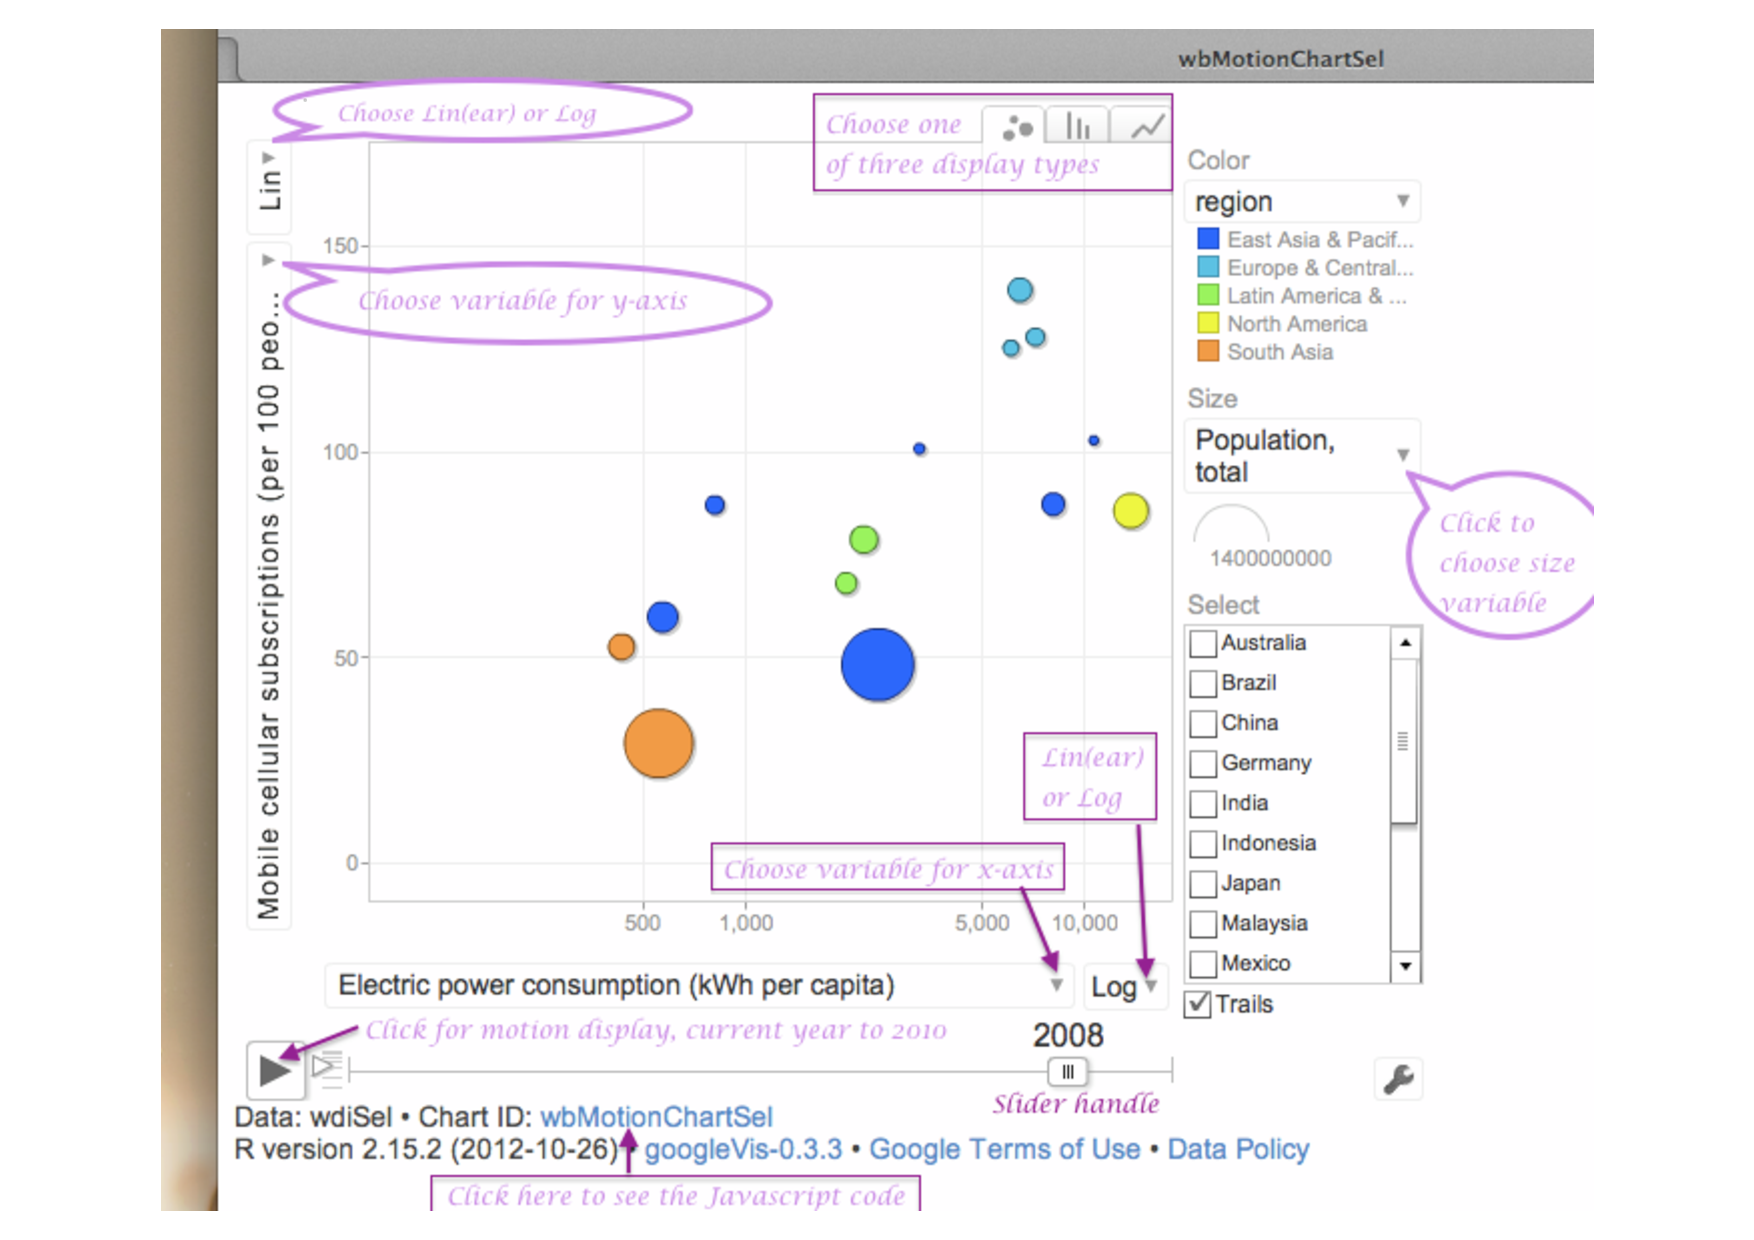
\includegraphics[scale=0.88]{colorArt/motionchart}}%
\caption{Snapshot of a motion chart, with annotation
  that identifies selected chart features that can be
  modified interactively.\label{col:mchart}}
\vspace*{-18pt}
\end{figure*}

\newpage
\subsection*{Florence Nightingale's Wedge Plot}\label{sec:wedge}

\marginnote[-24pt]{The name ``coxcomb'' arose from a misreading of
  Florence Nightingale's \textit{Mortality of the British Army} that
  was an annex to a larger official report. See {\small
    \url{http://www.york.ac.uk/depts/maths/histstat/small.htm}}}

Figure \ref{col:wedgeplot} is a ``wedge'' plot that shows the
mortality of British troops according to cause in the Crimean War over
1853-1853. It has often been called a ``coxcomb'' plot -- a name that
suits this imaginative form of graphical presentation.

\begin{figure*}
\centerline{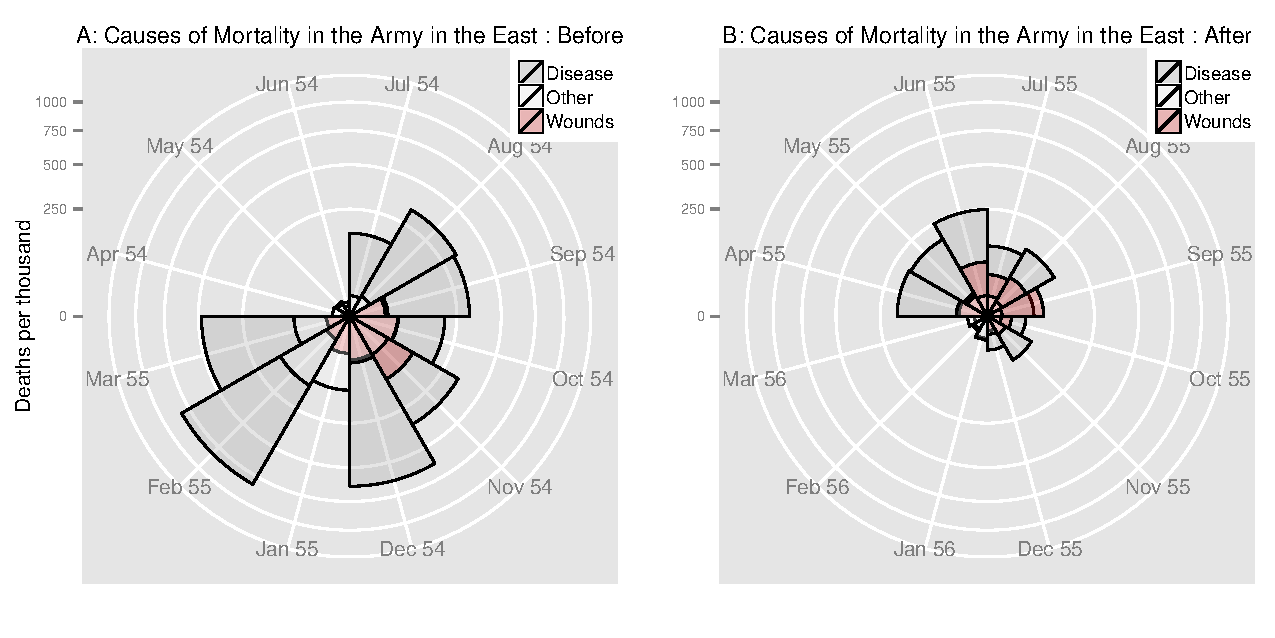
\includegraphics[width=0.97\textwidth]{colorArt/allwedge}}%
\caption{Deaths (per 1000 per annum), up to and after the
  Sanitary Commission's visit in March 1855.  Areas, measured from the
centres of the common vertices, are proportional
  to mortalities..\label{col:wedgeplot}}
\end{figure*}

Figure \ref{col:wedgeplot} is used here to show abilities in
\textit{ggplot2}.  The wedge plot is not ideal for giving an accurate
sense of the data.  It is not however easy to suggest an alternative
that is clearly better.

\subsection*{ Code for the wedge plot}

The url
\url{http://maths.anu.edu.au/~johnm/r/functions/wedgeORbubble.R}.\sidenote[][-1cm]{Data
  are from the data frame \txtt{Nightingale} in the {\em HistData}
  package. Subsection \ref{col:wedgeplot} showed how to create a
  dataset \txtt{Crimean} that is in a convenient form for creating
  this plot.} has code for the function \txtt{wedgeplot()} that was
used for this plot.  Note also the function \txtt{gdot()} that
gives a not entirely satisfactory alternative to the wedge plot.

\newpage
\subsection*{Selected base graphics parameter settings}
\begin{figure*}
\centerline{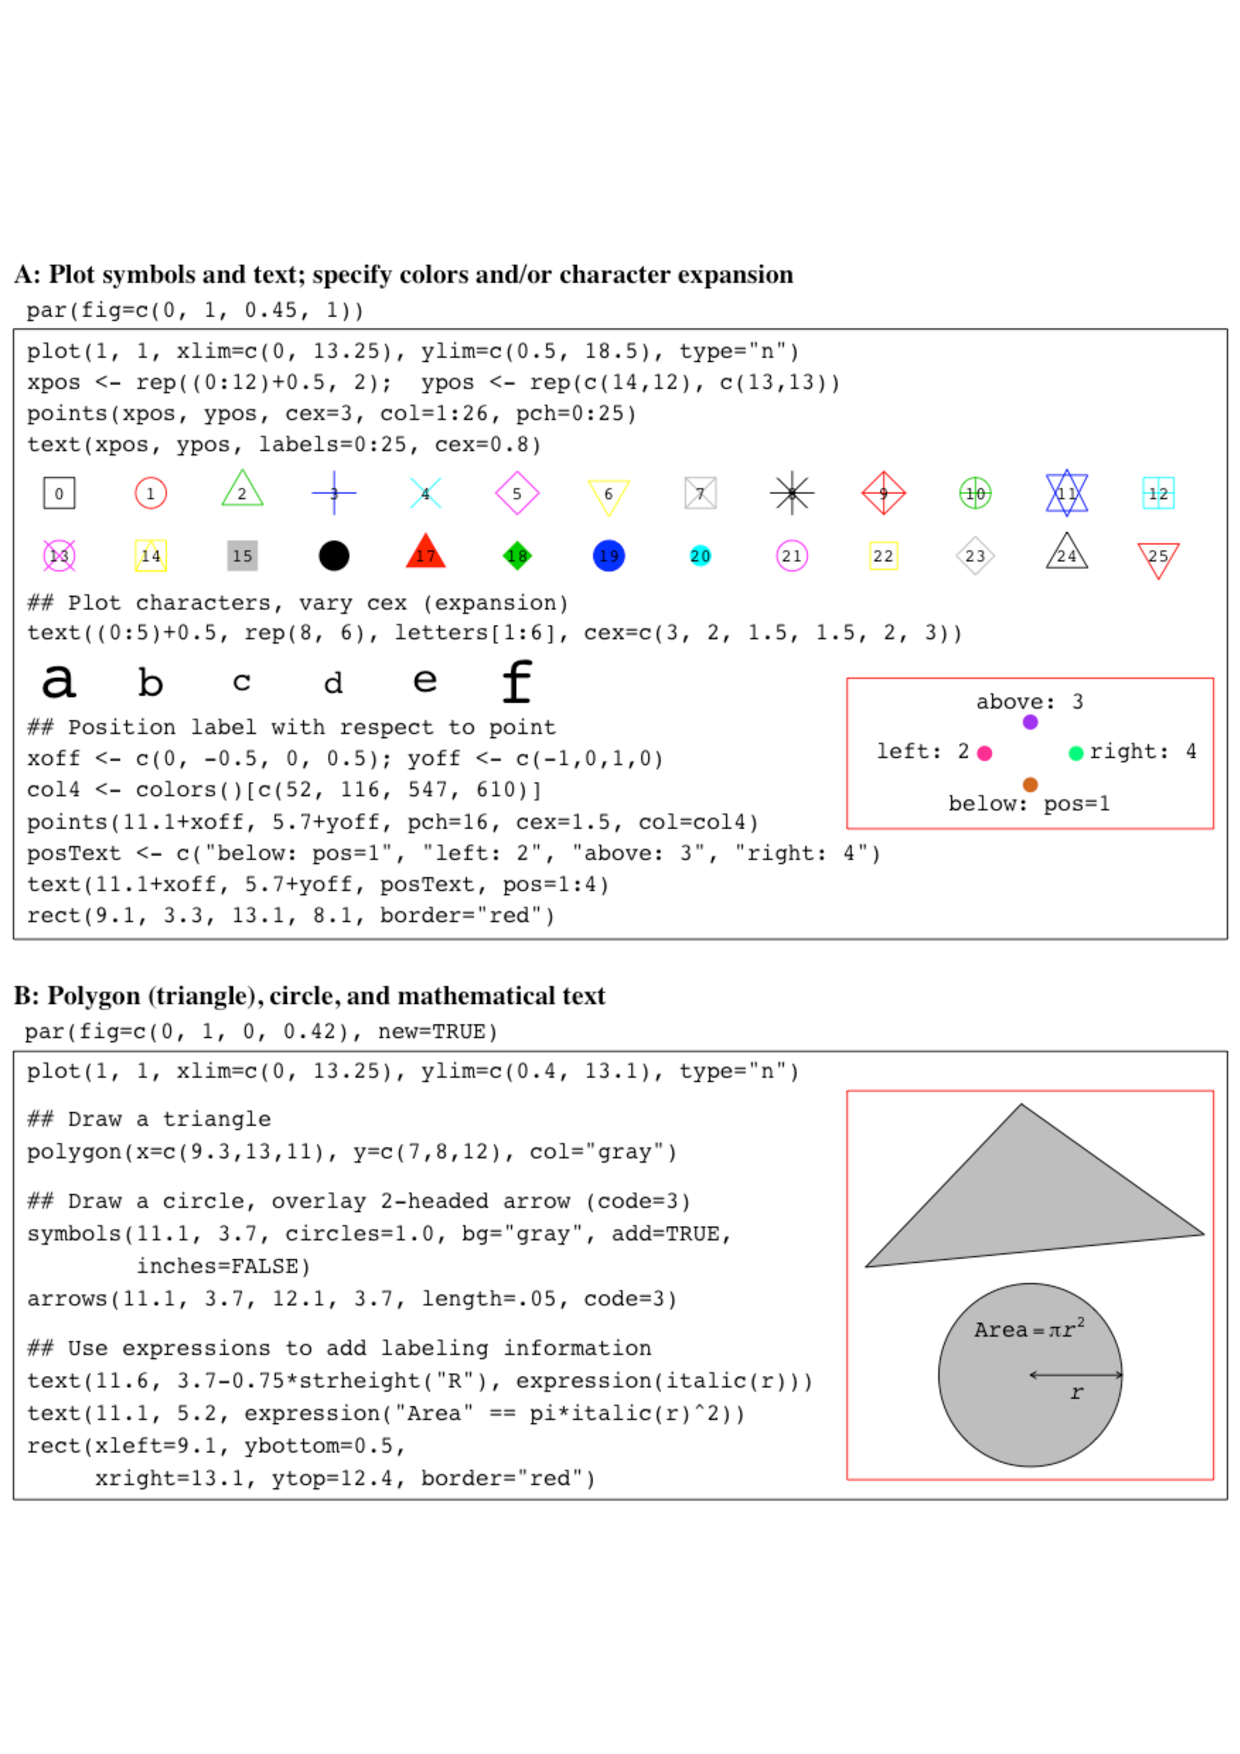
\includegraphics[width=0.85\textwidth]{colorArt/gphpars}}
\caption{This figure, intended to accompany Section \ref{ss:fine},
  demonstrates the use of parameter settings to control various
  graphical features.\label{fig:pars}}.
\end{figure*}

\vspace*{24pt}

\noindent
Note that the function \texttt{paste()}, used in line 5 of Panel A, turns the
  vector of numerical values \texttt{0:12} into a vector of character
  strings with elements \texttt{"0", "1", ..., "12"}.  An alternative to
\texttt{paste(0:12)} is \texttt{as.character(0:12)}.
\vfill
